% !Mode:: "TeX:UTF-8"
% !TEX root = ../main.tex
\chapter{多孔圆柱绕流的数值求解模型}

\section{问题描述}

\subsection{控制方程} % homogenous fluid region, and porous region

多孔圆柱绕流问题中的流动可以分为两部分:圆柱外为纯流体区域,圆柱内为多孔介质区域。在纯流体区域,不可压缩流动的质量守恒方程、动量守恒方程的微分形式分别为
\begin{gather}
	\nabla \cdot \bm{u} = 0 \\
	\frac{\partial(\rho\bm{u})}{\partial t} + \nabla \cdot (\rho\bm{u}\bm{u}) = -\nabla p + \mu\nabla^2\bm{u}
\end{gather}
\begin{tabularx}{\textwidth}{@{}l@{\quad}r@{——}X@{}}
	式中 & $\bm{u}$ & 速度;\\
		& $\rho$ & 密度;\\
		& $t$ & 时间;\\
		& $p$ & 压力;\\
		& $\mu$ & 动力粘性系数(动量扩散率)。
\end{tabularx}\vspace{3.15bp}

%积分形式为
%\begin{gather}
%	\frac{\partial}{\partial t}\int_{\Omega}\rho \diff\Omega = 
%\end{gather}

考虑多孔介质区域,控制方程采用 Darcy–Brinkman–Forchheimer 扩展模型:
\begin{gather}
	\nabla \cdot \bm{u} = 0 \\
	\frac{\partial(\rho\bm{u})}{\partial t} + 
	\nabla \cdot \left(\frac{\rho\bm{u}\bm{u}}{\varepsilon}\right) = 
	-\nabla (\varepsilon p^*) + \mu\nabla^2\bm{u} - 
	\frac{\mu\varepsilon}{K}\bm{u} - 
	\frac{\rho\varepsilon C_{\mathrm{F}}\abs{\bm{u}}}{\sqrt K}\bm{u}
\end{gather}
\begin{tabularx}{\textwidth}{@{}l@{\quad}r@{——}X@{}}
	式中 & $\bm{u}$ & 当地平均速度(达西速度);\\
		& $\varepsilon$ & 孔隙率;\\
		& $p^*$ & 内部平均压力;\\
		& $K$ & 渗透率;\\
		& $C_{\mathrm{F}}$ & Forchheimer 系数。
\end{tabularx}\vspace{3.15bp}
当地平均压力和内部平均压力之间存在关系 $p=\varepsilon p^*$,即 Dupuit–Forchheimer 关系。

\subsection{边界条件} % Including interface between the homogeneous fluid and porous medium regions

\section{离散方法}

\subsection{时间的离散}

\subsection{空间的离散}

\section{求解模型} %即求解器?SIMPLEC

纯流体区域。
用 $\phi$ 表示单位质量的某一守恒量,对于质量守恒,$\phi=1$,对于动量守恒,$\phi=\bm{u}$,对于其他标量的守恒,$\phi$ 表示单位质量内该标量的值。关于物理量 $\phi$ 积分形式的守恒方程为
\begin{equation}\label{eq: conservation}
	\frac{\partial}{\partial t}\int_{\varOmega}\rho\phi\diff\varOmega +
	\int_S\rho\phi\bm{u}\cdot\bm{n}\diff S =
	\int_S\varGamma\nabla\phi\cdot\bm{n}\diff S +
	\int_{\varOmega}q_{\phi}\diff\varOmega
\end{equation}
\begin{tabularx}{\textwidth}{@{}l@{\quad}r@{——}X@{}}
	式中 & $t$ & 时间;\\
		& $\varOmega$ & 控制体的体积;\\
		& $S$ & 控制体表面(控制面)的面积;\\
		& $\rho$ & 密度;\\
		& $\bm{u}$ & 速度;\\
		& $\bm{n}$ & 控制面某一点的单位法向量;\\
		& $\varGamma$ & 物理量 $\phi$ 的扩散率;\\
		& $q_{\phi}$ & 物理量 $\phi$ 的源或汇,即单位时间、单位体积的控制体内生成的 $\phi$。
\end{tabularx}\vspace{3.15bp}
假设控制体的中心点为 P,控制面分为东、南、西、北四部分,四个表面的中心点分别用字母 e、s、w、n 表示。方程中的四项分别表示随时间变化项、对流项、扩散项和源项,分别记为 $()$、$F^{\mathrm{c}}$、$F^{\mathrm{d}}$ 和 $Q_{\mathrm{P}}^{\phi}$。这样,公式 \eqref{eq: conservation} 可以简写为
\begin{equation}
	() + F^{\mathrm{c}} = F^{\mathrm{d}} + Q_{\mathrm{P}}^{\phi}
\end{equation}
下面将对方程中的每一项积分作出近似,近似方法参考 \cite{}。

(1)对流项的近似

图~ 是一个典型的二维控制体,将节点定义在每个控制体的中心位置。下面将以东边(east)为例。

质量流量为
\begin{equation}
	\dot m_{\mathrm{e}} = \int_{S_{\mathrm{e}}}\rho\bm{u}\cdot\bm{n}\diff S \approx 
	(\rho\bm{u}\cdot\bm{n})_{\mathrm{e}} S_{\mathrm{e}}
\end{equation}
表面的单位法向量 $\bm{n}_{\mathrm{e}}$ 定义为(重复的指标 $i$ 采用求和约定)
\begin{equation}
	\bm{n}_{\mathrm{e}}S_{\mathrm{e}} = S_{\mathrm{e}}^i \bm{i}_i = 
	(y_{\mathrm{ne}}-y_{\mathrm{se}})\bm{i} - (x_{\mathrm{ne}}-x_{\mathrm{se}})\bm{j}
\end{equation}
东边表面的面积 $S_{\mathrm{e}}$ 为
\begin{equation}
	S_{\mathrm{e}} = \sqrt{(S_{\mathrm{e}^x})^2 + (S_{\mathrm{e}^y})^2}
\end{equation}
于是,质量流量可以写为
\begin{equation}
	\dot m_{\mathrm{e}} = \rho_{\mathrm{e}}(S^x u_x + S^y u_y)_{\mathrm{e}}
\end{equation}
由此可见,非正交网格表面上的向量不是沿着坐标轴的方向,而是在两个坐标轴方向上均有分量,这个表面上的质量流量也同时跟两个坐标方向上的速度有关。

当表面上的质量流量已知时,物理量 $\phi$ 通过此表面的流率为
\begin{equation}
	F_{\mathrm{e}}^{\mathrm{c}} = \int_{S_{\mathrm{e}}}\rho\phi\bm{u}\cdot\bm{n}\diff S \approx \dot m_{\mathrm{e}} \phi_{\mathrm{e}}
\end{equation}
\begin{tabularx}{\textwidth}{@{}l@{\quad}r@{——}X@{}}
	式中 & $\phi_{\mathrm{e}}$ & 物理量 $\phi$ 在东边表面中心点处的值。
\end{tabularx}\vspace{3.15bp}
得到 $\phi_{\mathrm{e}}$ 最简单的办法是取相邻两个节点的平均值,这种方法将相邻两个节点的连线视为直线,如果线在表面处的方向发生转折,就会产生一个额外的误差。

(2)扩散项的近似

扩散项的流率为
\begin{equation}
	F_{\mathrm{e}}^{\mathrm{d}} = 
	\int_{S_{\mathrm{e}}}\varGamma\nabla\phi\cdot\bm{n}\diff S \approx
	(\varGamma\nabla\phi\cdot\bm{n})_{\mathrm{e}} S_{\mathrm{e}}
\end{equation}
物理量 $\phi$ 在东边表面中心点处的梯度在直角坐标系和当地坐标系下分别表示为
\begin{equation}
	\nabla\phi = 
	\frac{\partial\phi}{\partial x}\bm{i} + \frac{\partial\phi}{\partial y}\bm{j} = 
	\frac{\partial\phi}{\partial n}\bm{n} + \frac{\partial\phi}{\partial t}\bm{t}
\end{equation}
\begin{tabularx}{\textwidth}{@{}l@{\quad}r@{——}X@{}}
	式中 & $n,t$ & 坐标系在某一点的法向和切向。
\end{tabularx}\vspace{3.15bp}

如果 $\phi$ 在控制体表面的变化可以用一个形状函数来描述,那就可以求出这个函数在 e 位置对坐标轴各个方向的导数,接着可以得到扩散带来的流率:
\begin{equation}\label{eq: diffusive flux}
	F_{\mathrm{e}}^{\mathrm{d}} = \varGamma_{\mathrm{e}} \sum_i \left(\frac{\partial\phi}{\partial x_i}\right)_{\mathrm{e}} S_{\mathrm{e}}^i
\end{equation}
这样易于设为显式格式。

另一种方法是先得到控制体中心处的导数,然后再用插值的方法得到控制体表面处的值。首先用整个控制体上的平均值来近似中心处的值:
\begin{equation}
	\left(\frac{\partial\phi}{\partial x_i}\right)_{\mathrm{P}} \approx
	\frac{1}{\Delta\varOmega}\int_{\varOmega}\frac{\partial\phi}{\partial x_i}\diff\varOmega
\end{equation}
利用高斯公式将体积分转化为面积分:
\begin{equation}
	\int_{\varOmega}\frac{\partial\phi}{\partial x_i}\diff\varOmega =
	\int_S \phi\bm{i}_i\cdot\bm{n}\diff S \approx \sum_c\phi_c S_c^i,
	\quad c=\mathrm{e,s,w,n,\dots}
\end{equation}

上式表明,$\phi$ 在控制体中心对于 $x$ 的导数近似等于各个表面上 $\phi$ 和 $x$ 方向面积分量的乘积之和,即
\begin{equation}
	\left(\frac{\partial\phi}{\partial x_i}\right)_{\mathrm{P}} \approx
	\frac{1}{\Delta\varOmega}\sum_c\phi_c S_c^i
\end{equation}
这样,$\phi_c$ 可以使用和计算对流项时一样的值。如果在直角坐标系下使用线性插值,利用中心差分法也可以得到控制体中心位置的导数值:
\begin{equation}
	\left(\frac{\partial\phi}{\partial x_i}\right)_{\mathrm{P}} \approx
	\frac{\phi_{\mathrm{E}}-\phi_{\mathrm{W}}}{2\Delta x}
\end{equation}

对刚刚计算出的导数进行插值得到表面处的导数,然后根据式 \eqref{eq: diffusive flux} 可以得到所需的扩散流率。这种方法在迭代的过程中可能产生振荡解。

%隐式
选择固结于控制体表面中心位置的正交坐标系 $(n,t,s)$,可知扩散量仅由法向贡献:
\begin{equation}\label{eq: diffusive flux of local coordinate}
	F_{\mathrm{e}}^{\mathrm{d}} = \varGamma_{\mathrm{e}}\left(\frac{\partial\phi}{\partial n}\right)_{\mathrm{e}}S_{\mathrm{e}}
\end{equation}
使用中心差分,法向导数可以近似为?
\begin{equation}
	\left(\frac{\partial\phi}{\partial n}\right)_{\mathrm{e}} \approx
	\frac{\phi_{\mathrm{E}}-\phi_{\mathrm{P}}}{L_{\mathrm{PE}}}
\end{equation}
\begin{tabularx}{\textwidth}{@{}l@{\quad}r@{——}X@{}}
	式中 & $L_{\mathrm{PE}}$ & 相邻两个节点 E 和 P 之间的距离,$L_{\mathrm{PE}} = \abs{\bm{r}_{\mathrm{E}}-\bm{r}_{\mathrm{P}}}$。
\end{tabularx}\vspace{3.15bp}
如果是均匀的直角坐标系(当地的法向即为 $x$ 轴的方向),那么 $L_{\mathrm{PE}}=\Delta x$,于是
\begin{equation}
	\overline{\left(\frac{\partial\phi}{\partial n}\right)}_{\mathrm{e}} =
	\frac12\frac{\phi_{\mathrm{E}}-\phi_{\mathrm{W}}}{2\Delta x} +
	\frac12\frac{\phi_{\mathrm{EE}}-\phi_{\mathrm{P}}}{2\Delta x}
\end{equation}

从图~ 可以看出,当存在振荡时,由上式得出的 e 点导数值可能为零,但实际上该点具有较大的导数,振荡对迭代造成了影响。可以通过下面的方法避免:?
\begin{equation}
	F_{\mathrm{e}}^{\mathrm{d}} = F_{\mathrm{e}}^{\mathrm{d,impl}} +
	[F_{\mathrm{e}}^{\mathrm{d,expl}} - F_{\mathrm{e}}^{\mathrm{d,impl}}]^{\mathrm{old}}
\end{equation}
其中“impl”和“expl”分别代表隐式和显式形式的流率近似,“old”表示上次迭代的值。

Muzaferija\cite{} 提出了避免这一问题的有效方法。当连接 P、E 两点的线正交于控制体表面时,对 $n$ 的导数近似等于对 $\xi$ 的导数,$\xi$ 为连线的方向。公式 \eqref{eq: diffusive flux of local coordinate} 由隐式表达式近似:
\begin{equation}
	F_{\mathrm{e}}^{\mathrm{d}} = \varGamma_{\mathrm{e}}S_{\mathrm{e}}\left(\frac{\partial\phi}{\partial\xi}\right)_{\mathrm{e}} = 
	\varGamma_{\mathrm{e}}S_{\mathrm{e}}\frac{\phi_{\mathrm{E}}-\phi_{\mathrm{P}}}{L_{\mathrm{PE}}}
\end{equation}
如果 P、E 的连线正交于单元表面,这是一个具有二阶精度的方法,并且延迟校正项必须为零。?当网格是非正交时,延迟校正项必须包括 $\xi$ 和 $n$ 两个方向导数的差值。Muzaferija\cite{} 提出的校正格式为
\begin{equation}\label{eq: Muzaferija1994 formula}
	F_{\mathrm{e}}^{\mathrm{d}} = \varGamma_{\mathrm{e}}S_{\mathrm{e}}\left(\frac{\partial\phi}{\partial\xi}\right)_{\mathrm{e}} +
	\varGamma_{\mathrm{e}}S_{\mathrm{e}}\left[ 
	\overline{\left(\frac{\partial\phi}{\partial n}\right)}_{\mathrm{e}} - 
	\overline{\left(\frac{\partial\phi}{\partial\xi}\right)}_{\mathrm{e}} \right]^{\mathrm{old}}
\end{equation}
等式右边的第一项以隐式处理,第二项为延迟校正项。校正项使用单元中心处的导数来插值:
\begin{equation}
	\overline{\left(\frac{\partial\phi}{\partial n}\right)}_{\mathrm{e}} =
	\overline{(\nabla\phi)}_{\mathrm{e}}\cdot\bm{n}; \quad
	\overline{\left(\frac{\partial\phi}{\partial\xi}\right)}_{\mathrm{e}} =
	\overline{(\nabla\phi)}_{\mathrm{e}}\cdot\bm{i}_{\xi}
\end{equation}
其中 $\bm{i}_{\xi}$ 为 $\xi$ 方向的单位向量。最终得到的扩散流率的表达式为
\begin{equation}
	F_{\mathrm{e}}^{\mathrm{d}} = \varGamma_{\mathrm{e}}S_{\mathrm{e}}\frac{\phi_{\mathrm{E}}-\phi_{\mathrm{P}}}{L_{\mathrm{PE}}} +
	\varGamma_{\mathrm{e}}S_{\mathrm{e}}\overline{(\nabla\phi)}_{\mathrm{e}}^{\mathrm{old}}\cdot(\bm{n}-\bm{i}_{\xi})
\end{equation}
当 $\bm{i}_{\xi}=\bm{n}$ 时,上式退化为正交时的情形。

在以上的方法中,我们假设 P、E 间的连线通过了单元东边表面的中心 e。以上的面积分具有二阶精度。如果网格是不规则的,P、E 连线可能不会经过表面的中心点,前面公式中的 $\phi_{\mathrm{e}}$ 和 $(\partial\phi/\partial\xi)_{\mathrm{e}}$ 等并不是 e 点的值,而是 P、E 连线与表面的交点 $\mathrm{e}'$ 处的值,如图~ 所示。e 和 $\mathrm{e}'$ 之间的差别带来了误差,使得原来的面积分不再具有二阶精度,误差可能会使精度降为一阶。

控制体表面中心处 e 点的值可以通过辅助节点 $\mathrm{P}'$ 和 $\mathrm{E}'$ 得到,$\mathrm{P}'$、$\mathrm{E}'$ 的连线通过 e 点并指向 e 点的法向,$\mathrm{P}'$ 和 $\mathrm{E}'$ 分别位于 P、N 以及 E、NE 的连线上,如图~ 所示。隐式项基于节点 P 和 E 处的值,忽略网格的不规则(即使用 $\mathrm{e}'$ 点的值),对隐式项和更精确的方法之间的差值进行显式处理。于是,公式 \eqref{eq: Muzaferija1994 formula} 被修正为
\begin{equation}
	F_{\mathrm{e}}^{\mathrm{d}} = \varGamma_{\mathrm{e}}S_{\mathrm{e}}\left(\frac{\partial\phi}{\partial\xi}\right)_{\mathrm{e'}} +
	\varGamma_{\mathrm{e}}S_{\mathrm{e}}\left[ 
	\overline{\left(\frac{\partial\phi}{\partial n}\right)}_{\mathrm{e}} - 
	\overline{\left(\frac{\partial\phi}{\partial\xi}\right)}_{\mathrm{e'}} \right]^{\mathrm{old}}
\end{equation}
控制体表面中心处的法向导数使用中心差分计算:
\begin{equation}
	\left(\frac{\partial\phi}{\partial n}\right)_{\mathrm{e}} \approx
	\frac{\phi_{\mathrm{E'}}-\phi_{\mathrm{P'}}}{L_{\mathrm{P'E'}}}
\end{equation}
其中 $L_{\mathrm{P'E'}}$ 为 $\mathrm{P}'$ 和 $\mathrm{E}'$ 两点之间的距离,$L_{\mathrm{P'E'}} = \abs{\bm{r}_{\mathrm{E'}}-\bm{r}_{\mathrm{P'}}}$。$\phi_{\mathrm{E'}}$ 和 $\phi_{\mathrm{P'}}$的值可以使用线性插值来计算,或者通过控制体中心处的梯度得到:
\begin{equation}
	\phi_{\mathrm{P'}} = \phi_{\mathrm{P}} + (\nabla\phi)_{\mathrm{P}}\cdot(\bm{r}_{\mathrm{P'}}-\bm{r}_{\mathrm{P}})
\end{equation}
上面是具有二阶精度的最简单格式。

(3)源项的近似

整个控制体内产生的源可以近似为控制体中心点的值与控制体体积的乘积:
\begin{equation}
	Q_{\mathrm{P}}^{\phi} = \int_{\varOmega}q_{\phi}\diff\varOmega \approx
	q_{\phi,\mathrm{P}}\Delta\varOmega
\end{equation}
上式具有二阶精度。

对于结构化网格,二维四边形网格形成的控制体的体积等于两条对角线向量积的一半:
\begin{equation}
\begin{split}
	\Delta\varOmega &= \frac12\abs{(\bm{r}_{\mathrm{ne}}-\bm{r}_{\mathrm{sw}})\times (\bm{r}_{\mathrm{nw}}-\bm{r}_{\mathrm{se}})} \\
	&=\frac12[(x_{\mathrm{ne}}-x_{\mathrm{sw}})(y_{\mathrm{nw}}-y_{\mathrm{se}}) - (y_{\mathrm{ne}}-y_{\mathrm{sw}})(x_{\mathrm{nw}}-x_{\mathrm{se}})]
\end{split}
\end{equation}
其中 $\bm{r}_{\mathrm{ne}}$ 是“ne”点的位置向量,其他同理。

对于动量方程中的压力项,既可以将其视为作用于控制体表面的保守力,也可以视为非保守的体积力。如视为表面力,
\begin{equation}
\begin{split}
	Q_{\mathrm{P}}^p &= -\int_S p\bm{i}\cdot\bm{n}\diff S \approx
	\sum_c p_cS_c^x \\
	&= -p_{\mathrm{e}}(y_{\mathrm{ne}}-y_{\mathrm{se}}) +
	p_{\mathrm{w}}(y_{\mathrm{nw}}-y_{\mathrm{sw}}) +
	p_{\mathrm{n}}(y_{\mathrm{ne}}-y_{\mathrm{nw}}) -
	p_{\mathrm{s}}(y_{\mathrm{se}}-y_{\mathrm{sw}})
\end{split}
\end{equation}
如视为体积力,
\begin{equation}
	Q_{\mathrm{P}}^p = 
	-\int_{\varOmega} \frac{\partial p}{\partial x} \diff\varOmega \approx 
	-\left(\frac{\partial p}{\partial x}\right)_{\mathrm{P}} \Delta\varOmega
\end{equation}
第一种方法是完全守恒的,如果导数 $\partial p/\partial x$ 是使用高斯定理计算的话,第二种方法也是守恒的:两者通过高斯定理相联系。?如果压力梯度不在直角坐标系下表示,而在位于控制体中心的当地坐标系 $(\xi,\eta)$ 下表示,那么?
\begin{equation}
	Q_{\mathrm{P}}^p \approx 
	-(p_{\mathrm{e}}-p_{\mathrm{w}})(y_{\mathrm{n}}-y_{\mathrm{s}}) + 
	(p_{\mathrm{n}}-p_{\mathrm{s}})(y_{\mathrm{e}}-y_{\mathrm{w}})
\end{equation}
由此得出了动量方程中压力项的近似计算。

通过以上各项的近似,水平方向的(动量?)方程离散之后可以写为
\begin{equation}
	\frac{\partial}{\partial t}\int_{\varOmega}\rho\phi\diff\varOmega +
	A_{\mathrm{P}}\phi_{\mathrm{P}} + \sum_l A_l\phi_l = Q_{\mathrm{P}}^* - \left(\frac{\partial p}{\partial x}\right) \Delta\varOmega
\end{equation}
上式以各个节点的 $\phi$ 为未知量,通过求解代数方程组得到,压力项通过 SIMPLEC 算法求解?\cite{}
\begin{equation}
	u_{\mathrm{e}}^{\mathrm{m}} = \overline{(u^m)}_{\mathrm{e}} - \Delta\varOmega \overline{\left(\frac{1}{A_{\mathrm{P}}^u+\sum_lA_l^u}\right)}_{\mathrm{e}} \left[\left(\frac{\partial p}{\partial x}\right)_{\mathrm{e}}-\overline{\left(\frac{\partial p}{\partial x}\right)}_{\mathrm{e}}\right]^{m-1}
\end{equation}

多孔介质区域。
控制方程与纯流体区域相似,离散方法也相似。


\begin{equation}
	F_{\mathrm{e}}^{\mathrm{c}} = 
\end{equation}

\section{网格划分}
 
\subsection{网格生成}

流动区域设定为边长 60 的正方形。为了获得圆柱内外的流动状态,流动区域被划分为三块,其中有两块位于圆柱内部,一块位于圆柱外部,见图~\ref{fig: grid}。网格尺寸见表~\ref{tab: grid}。雷诺数和达西数分别为 100 和 0.0001。
\begin{figure}
	\centering
	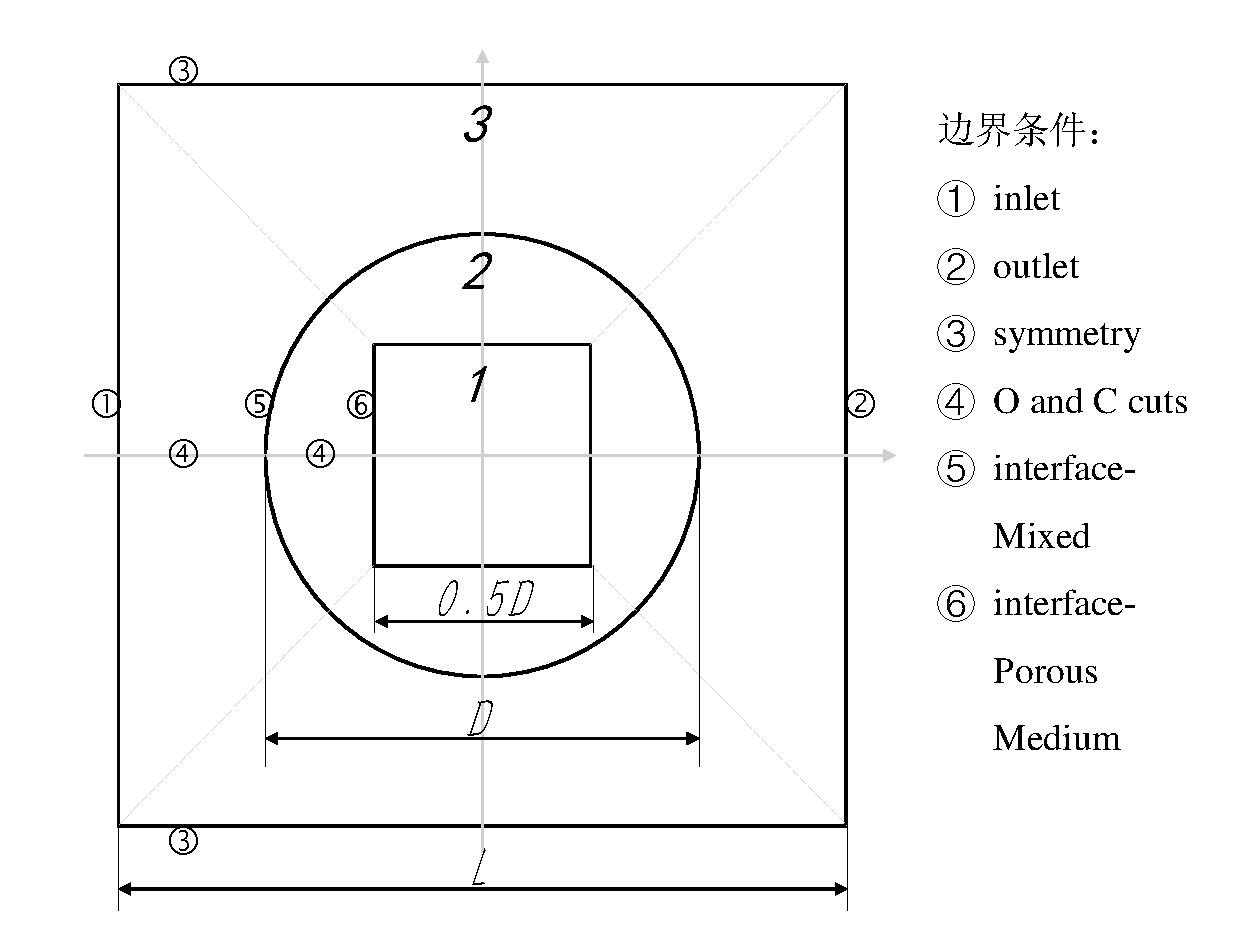
\includegraphics[scale=.6]{../diagrams/grid}
	\caption{网格划分}\label{fig: grid}
\end{figure}

\subsection{网格无关性分析}

\begin{table}
	\caption{网格尺寸}\label{tab: grid}
	\vspace{.5em}\centering\wuhao
	\begin{tabular}{ccccc}
		\toprule[1.5pt]
		\multirow{2}[3]{*}{序号} & \multicolumn{3}{c}{网格尺寸} & \multirow{2}[3]{*}{平均阻力系数} \\
		\cmidrule[.67pt](lr){2-4}
		& Block 1 & Block 2 & Block 3 & \\
		\midrule[1pt]
		1 & 40 $\times$ 40 & 160 $\times$ 25 & 160 $\times$ 140 & 1.2354 \\
		2 & 60 $\times$ 60 & 240 $\times$ 30 & 240 $\times$ 170 & 1.2426 \\
		3 & 80 $\times$ 80 & 320 $\times$ 40 & 320 $\times$ 200 & 1.2462 \\
		4 & 100 $\times$ 100 & 400 $\times$ 50 & 400 $\times$ 230 & 1.2417 \\
		\bottomrule[1.5pt]
	\end{tabular}
\end{table}

\section{结果验证}

\section{本章小结}
